%!TEX root=../../main.tex

%_______________
\section{Exercises}
\label{ch3Exercises}


%_______________
%\subsection{Variability in estimates}

% 1 oi_biostat, blue_eggs

\eoce{\qt{Egg coloration\label{blue_eggs}} The evolutionary role of variation in bird egg coloration remains mysterious to biologists. One hypothesis suggests that egg color may play a role in sexual selection. For example, perhaps healthier females are able to deposit more blue-green pigment into eggshells instead of using it themselves as an antioxidant. Researchers measured the blue-green chroma (BGC) of 70 different collared flycatcher nests in an area of the Czech Republic.
	
	\begin{minipage}[c]{0.75\textwidth}
		\begin{center}
			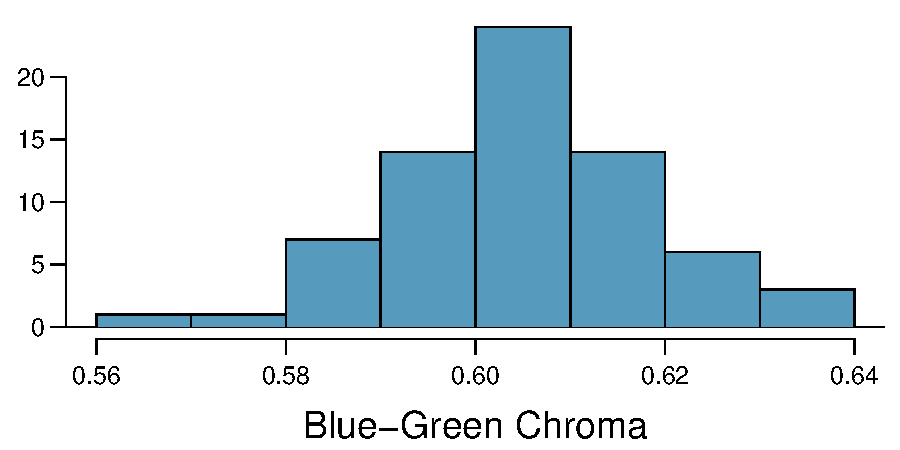
\includegraphics[width=\textwidth]{ch_03a_inference_foundations_oi_biostat/figures/eoce/blue_eggs/blue_eggs_hist.pdf}
		\end{center}
	\end{minipage}
	\begin{minipage}[c]{0.22\textwidth}
		\begin{center}
			\begin{tabular}{l|r l}
				Min     & 0.5675 \\
				Q1      & 0.5977 \\
				Median  & 0.6046 \\
				Mean    & 0.6052 \\
				SD      & 0.0131 \\
				Q3      & 0.6126 \\
				Max     & 0.6355 \\
			\end{tabular}
		\end{center}
	\end{minipage}	
	\begin{parts}
		\item What is the point estimate for the average BGC of nests?
		\item What is the point estimate for the standard deviation of the BGC of eggs across nests?
		\item Would a nest with average BGC of 0.63 be considered unusually high? Explain your reasoning.
		\item Compute the standard error of the sample mean using the summary statistics.
	\end{parts}
}{}
